\chapter{Validazione (parte 3): errori tipici e FAQ}\label{ch-11}

L'ultima parte sulla validazione raccoglie consigli pratici sull'uso
della cross-validation, gli \textbf{errori più frequenti} (soprattutto
nei progetti) e alcuni esempi di model selection, in parte tratti dalle
slide di Andrew W. Moore (CMU).

\section{Arresto dell'addestramento}\label{arresto-delladdestramento}

\subsection{Non fissare un numero arbitrario di
epoche}\label{non-fissare-un-numero-arbitrario-di-epoche}

\begin{boxwarning}{Errore frequente}

Evitare di fermare l'addestramento di una rete dopo un \textbf{numero
fisso e arbitrario di epoche}.

\end{boxwarning}

Perché:

\begin{itemize}
\tightlist
\item
  se è piccolo, ci si può fermare \textbf{troppo presto} (underfitting,
  o si favoriscono i learning rate alti che richiedono meno epoche);
\item
  se è grande, ci si può fermare \textbf{troppo tardi} (overfitting o
  tempo perso);
\item
  non può andare bene lo stesso valore per tutte le configurazioni e le
  iterazioni di una K-fold CV;
\item
  e quale numero usare nel riaddestramento finale?
\end{itemize}

Anche \textbf{selezionare il numero di epoche tramite model selection}
non è la pratica migliore: è meglio di un numero fisso ma ancora
impreciso (per i problemi con la K-fold CV e perché esistono criteri
migliori). Le soluzioni che funzionano bene con un sistema \textbf{ben
regolarizzato} sono quelle viste in
\href{08\%20-\%20Reti\%20neurali\%20(parte\%202)\%20-\%20addestramento\%20in\%20pratica}{08
- Reti neurali (parte 2) - addestramento in pratica}: guardare la
convergenza del training (soglia sulla diminuzione dell'errore o sul
gradiente), oppure l'\textbf{early stopping} se si può/vuole usare un
validation set.

\subsection{Early stopping}\label{early-stopping}

\begin{boxwarning}{Early stopping e model selection}

Il criterio di early stopping (ES) fa \textbf{parte della model
selection} (non va applicato sul TS): in linea di principio richiede un
\textbf{VL set ogni volta} che si addestra il modello.

\end{boxwarning}

È delicato: usa parte dei dati solo per decidere quando fermarsi, senza
dare un valore concreto di iperparametro, e può diventare complesso
dentro una CV. Il problema: come scegliere il punto di arresto per il
\textbf{riaddestramento finale}, se ogni fold della CV ha un punto di
arresto diverso?

\begin{itemize}
\tightlist
\item
  Si potrebbe considerare il numero di epoche come iperparametro e
  prendere la \textbf{media} sui fold. Ma cambiando la quantità di dati
  nel riaddestramento il punto di arresto ottimo può cambiare (ad
  esempio con più dati per epoca, e quindi più aggiornamenti per epoca
  in on-line, servono meno epoche): si rischia sotto- o
  sovra-addestramento.
\item
  \textbf{Molto meglio}: prendere la \textbf{media dell'errore di
  training} nel punto migliore di validazione e usarla come soglia nel
  riaddestramento, per raggiungere lo stesso livello di fitting
  (evitando effetti di sotto-addestramento).
\item
  Altrimenti serve un VL set ogni volta: ad esempio CV con ES attivo in
  ogni fold di validazione (insieme agli altri iperparametri); trovati i
  migliori iperparametri, si riaddestra sul dataset ricomposto usando
  ancora una parte dei dati come VL per l'ES.
\end{itemize}

È una scelta: usare l'ES oppure affidarsi a \textbf{modelli
regolarizzati} con criteri di arresto standard (es. nessun miglioramento
sul training). In ogni caso la regolarizzazione aiuta a evitare un forte
sovra-addestramento e riduce la dipendenza dall'ES.

\section{Inizializzazione casuale e model
selection}\label{inizializzazione-casuale-e-model-selection}

Inizializzazioni diverse dei pesi portano a \textbf{modelli diversi}.
Come scegliere quello finale (scelta che va riportata nel report)?

\begin{itemize}
\tightlist
\item
  Si calcolano \textbf{media e varianza} dell'errore/accuratezza sulle
  diverse prove: un caso casuale cadrà in quell'intervallo, quindi il
  rischio è sotto controllo, a meno di una varianza alta (che comunque è
  un segnale negativo, vedi la lezione su bias e varianza).
\item
  Si possono usare \textbf{tutti} i modelli, con un \textbf{ensemble}
  (media delle uscite o voto).
\item
  Se se ne sceglie \textbf{uno}, quella è una \textbf{model selection} e
  serve un VL set: il \textbf{migliore} (errore minimo sul VL), la
  \textbf{mediana} (scelta più cauta), oppure uno \textbf{casuale} (in
  questo caso non serve un VL set).
\item
  Si possono anche scartare i casi ``sfortunati'' guardando solo
  l'errore di training.
\end{itemize}

\section{Selezione sequenziale degli
iperparametri}\label{selezione-sequenziale-degli-iperparametri}

\begin{boxwarning}{Errore frequente}

Selezionare gli iperparametri \textbf{uno alla volta}, in sequenza,
introduce un \textbf{bias legato all'ordine}. Esempio: scegliere il
miglior \(\eta\) con 10 unità e poi usarlo anche con 100 unità.

\end{boxwarning}

Il procedimento corretto:

\begin{enumerate}
\def\labelenumi{\arabic{enumi}.}
\tightlist
\item
  prove iniziali per determinare gli \textbf{intervalli} giusti (ad
  esempio guardando la stabilità del training) e gli iperparametri più
  \textbf{influenti} (ad esempio guardando la varianza dei risultati);
\item
  ricerca su una \textbf{griglia con tutte le combinazioni} degli
  iperparametri (più iperparametri e valori → tabella più grande);
\item
  eventuali griglie \textbf{annidate}, da grossolane a fini, su
  intervalli sempre più piccoli, ma considerando \textbf{tutti gli
  iperparametri significativi insieme}, per tenere conto degli effetti
  incrociati.
\end{enumerate}

Ma: ragionare, selezionare gli aspetti rilevanti, non affidarsi solo ad
approcci automatici sistematici e costosi. I vincoli di tempo del
progetto dovrebbero spingere verso schemi semplici e veloci, ma corretti
e ragionevoli.

\section{Cosa fare dopo selezione e
valutazione?}\label{cosa-fare-dopo-selezione-e-valutazione}

\begin{boxquestion}{Posso riprogettare il modello in base al risultato sul test?}

No: non è il modo corretto e non è davvero vantaggioso (a meno di avere
nuovi dati per un nuovo test set). Ripetendo questo procedimento sugli
stessi dati si può ottenere qualunque risultato si voglia, adattando il
modello a quel dataset: il modello può diventare perfetto su di esso e
non nell'uso futuro, e \textbf{non si sta più stimando il rischio}.

\emph{Non bisogna regolare il predittore (a mano o automaticamente)
sulla base dell'errore di test, perché non potremmo farlo sugli esempi
futuri.} Nelle competizioni il blind test impedisce proprio questo. La
valutazione su un test interno resta comunque utile per
\textbf{verificare il proprio approccio}.

\end{boxquestion}

La tentazione di decidere in base ai risultati è un problema
``psicologico'', esterno ai metodi di ML. Almeno esserne consapevoli,
oppure meglio:

\begin{itemize}
\tightlist
\item
  per fare un \textbf{buon modello} bisogna fare una \textbf{buona model
  selection};
\item
  per stimare le \textbf{prestazioni reali} bisogna fare una stima
  \textbf{rigorosa} sul test.
\end{itemize}

\section{La cross-validation può andare in
overfitting}\label{la-cross-validation-puuxf2-andare-in-overfitting}

Un uso intensivo della cross-validation può portare a overfitting?
\textbf{Sì}, e conserva i problemi già visti. Esempio con la feature
selection:

\begin{itemize}
\tightlist
\item
  dataset con 20--30 record e 1000 attributi;
\item
  si provano 1000 modelli di regressione lineare, ognuno con un solo
  attributo;
\item
  il migliore dei 1000 sembra buono (sul validation set)\ldots{} ma
  sarebbe sembrato buono anche con un output \textbf{puramente casuale}!
\end{itemize}

Oppure (uso sbagliato): approssimando un target casuale si trova, con
una K-fold CV per il test, un errore del 3\% invece del vero 50\%, dopo
aver scelto le feature per miglior correlazione con i target.
\textbf{Perché?} La selezione è stata fatta su \textbf{tutti} gli
esempi.

Cosa fare? Tenere da parte i campioni \textbf{prima} di selezionare:

\begin{itemize}
\tightlist
\item
  tenere un \textbf{test set aggiuntivo} prima di qualsiasi model
  selection e verificare che il modello migliore funzioni bene anche su
  di esso;
\item
  per la model selection con CV: usare ``\textbf{CV + test}'' o la
  \textbf{double CV} (rifacendo la selezione per ogni fold);
\item
  per l'assessment con CV: fare la \textbf{feature selection dentro ogni
  fold}. Così si ottiene la stima corretta, circa il 50\% per il task
  casuale.
\end{itemize}

\section{Quale cross-validation?}\label{quale-cross-validation}

{\def\LTcaptype{none} % do not increment counter
\begin{longtable}[]{@{}
  >{\raggedright\arraybackslash}p{(\linewidth - 4\tabcolsep) * \real{0.3333}}
  >{\raggedright\arraybackslash}p{(\linewidth - 4\tabcolsep) * \real{0.3333}}
  >{\raggedright\arraybackslash}p{(\linewidth - 4\tabcolsep) * \real{0.3333}}@{}}
\toprule\noalign{}
\begin{minipage}[b]{\linewidth}\raggedright
\end{minipage} & \begin{minipage}[b]{\linewidth}\raggedright
Svantaggi
\end{minipage} & \begin{minipage}[b]{\linewidth}\raggedright
Vantaggi
\end{minipage} \\
\midrule\noalign{}
\endhead
\bottomrule\noalign{}
\endlastfoot
\textbf{Test set (hold-out)} & varianza: stima inaffidabile delle
prestazioni future (fortuna/sfortuna) & economico \\
\textbf{Leave-one-out} & costoso; ha comportamenti strani & non spreca
dati \\
\textbf{10-fold} & spreca il 10\% dei dati; 10 volte più costoso del
test set & spreca solo il 10\%; solo 10 volte più costoso invece di
\(R\) volte \\
\textbf{3-fold} & spreca più dati del 10-fold; più costoso del test set
& leggermente meglio del test set \\
\textbf{R-fold} (\(R = l\)) & identico al leave-one-out & \\
\end{longtable}
}

\section{Esempi di model selection}\label{esempi-di-model-selection}

\subsection{Esempio 1: modelli diversi}\label{esempio-1-modelli-diversi}

\begin{figure}[htbp]
\centering
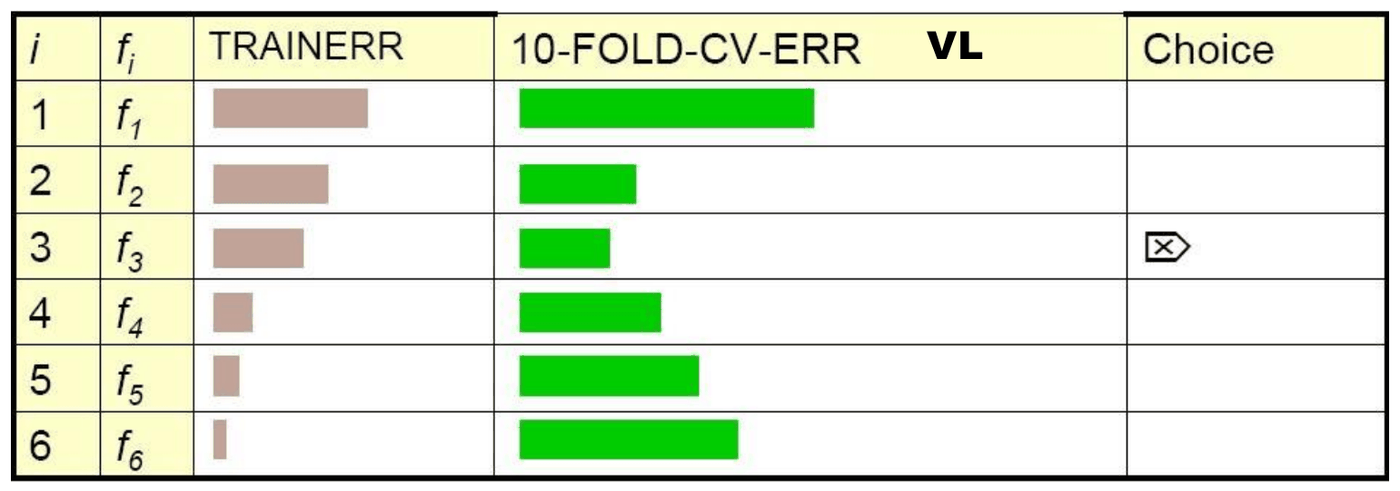
\includegraphics[width=0.86\linewidth,height=0.42\textheight,keepaspectratio]{images/11-val3_es-modelli.png}
\caption{Scelta tra sei classi di modelli con la 10-fold CV.}
\end{figure}

Si sceglie la classe di modelli con il \textbf{miglior punteggio di CV},
la si riaddestra su tutti i dati, e quello è il modello predittivo da
usare. La scelta si fa guardando \textbf{solo l'errore di validazione},
\textbf{non} l'errore di training (né una media dei due).

\subsection{Esempio 2: numero di unità
nascoste}\label{esempio-2-numero-di-unituxe0-nascoste}

\begin{figure}[htbp]
\centering
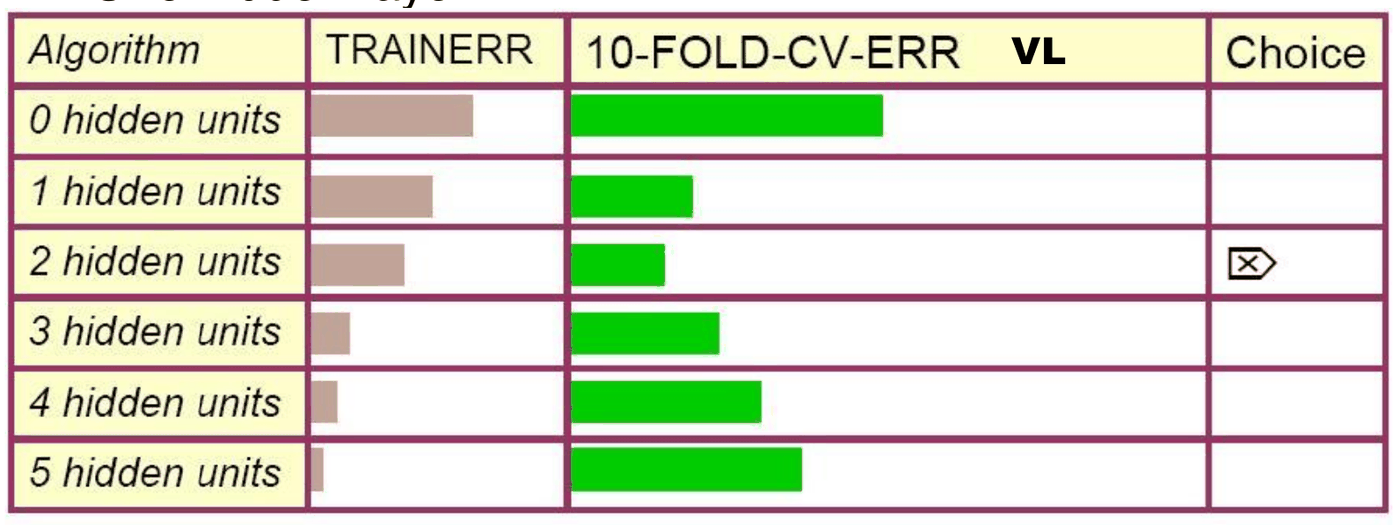
\includegraphics[width=0.86\linewidth,height=0.42\textheight,keepaspectratio]{images/11-val3_es-unita.png}
\caption{Scelta del numero di unità nascoste di una rete con uno strato nascosto.}
\end{figure}

L'errore di training decresce sempre con il numero di unità, ma l'errore
di CV ha un minimo (qui 2 unità). Nella pratica la ricerca si fa su
valori come 10, 20, 30\ldots{} (o con altri passi).

\subsection{Esempio 3: K-NN}\label{esempio-3-k-nn}

\begin{figure}[htbp]
\centering
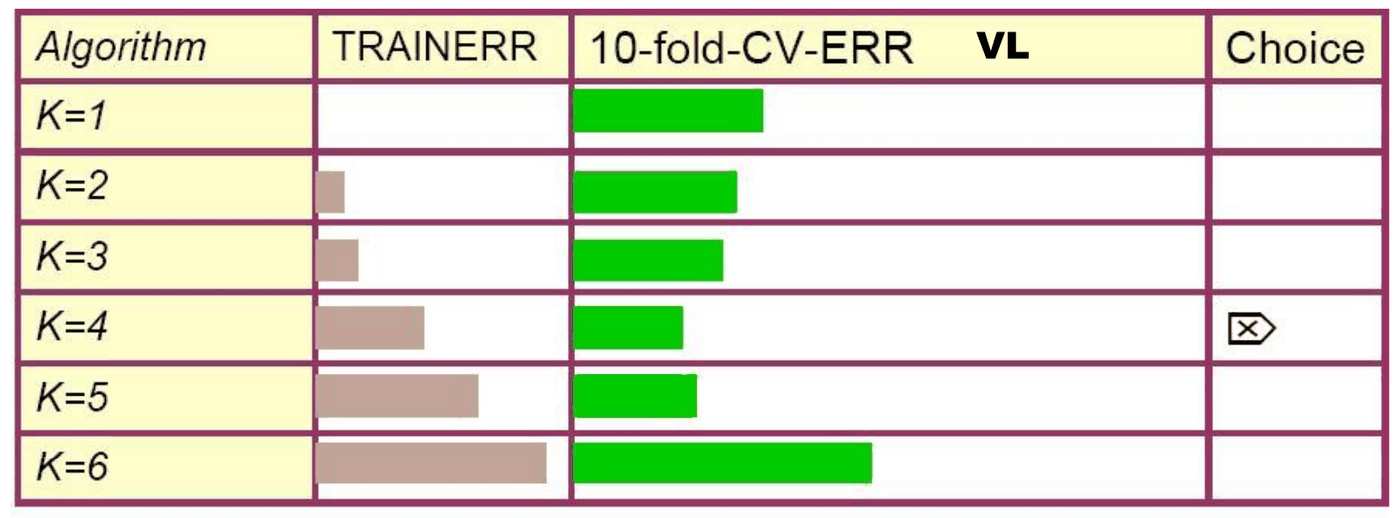
\includegraphics[width=0.86\linewidth,height=0.42\textheight,keepaspectratio]{images/11-val3_es-knn.png}
\caption{Scelta di \(k\) per il K-NN con leave-one-out CV.}
\end{figure}

Perché la \textbf{leave-one-out} per il K-NN e la 10-fold per le reti?
Per ragioni \textbf{computazionali}: per il K-NN (e gli altri metodi non
parametrici) la LOOCV costa quanto una normale predizione (non c'è un
modello da addestrare). E perché fermarsi a \(K = 6\)? Solo perché le
cose sembravano peggiorare al crescere di \(K\); e non c'è garanzia che
un ottimo locale di \(K\) rispetto alla LOOCV sia quello globale (la
relazione può essere molto irregolare). Per esplorare molti valori si
possono usare valori a crescita esponenziale
(\(K = 1, 2, 4, 8, 16, \dots\)) o una ricerca \emph{hill-climbing}
partendo da un valore iniziale.

\section{Conclusioni pratiche}\label{conclusioni-pratiche}

\begin{itemize}
\tightlist
\item
  L'\textbf{hold-out semplice} è molto usato: a volte il test set è già
  dato separatamente o ``preso'' da applicazioni precedenti. Attenzione
  con pochi dati e controllare i tassi d'errore su TR e VL.
\item
  La \textbf{5- o 10-fold CV} è raccomandata come buon compromesso (tra
  bias e varianza della stima) rispetto alla leave-one-out (Hastie et
  al.).
\end{itemize}

Nella prossima lezione si torna alla stima \textbf{analitica}
dell'errore atteso, con la Structural Risk Minimization e la
VC-dimension: offre spunti interessanti per la selezione e il confronto
tra modelli (dove conta la \textbf{dimensione relativa} degli errori),
in alternativa alla valutazione puramente empirica.

\begin{boxquestion}{Possibili domande d'esame}

\begin{itemize}
\tightlist
\item
  Perché non bisogna fermare l'addestramento dopo un numero fisso di
  epoche?
\item
  Come si gestisce l'early stopping con la cross-validation e il
  riaddestramento finale?
\item
  Come scegliere il modello finale con più inizializzazioni casuali?
\item
  Cos'è l'errore della selezione sequenziale degli iperparametri?
\item
  La cross-validation può andare in overfitting? Come evitarlo?
\item
  Confrontare hold-out, K-fold e leave-one-out.
\end{itemize}

\end{boxquestion}
